\chapter{Model}\label{cha:model}

 This model is inspired by Ejenstams work \cite{ejenstam_2014}. That model is centered around work performed in fixtures. So tasks can easily be labeled \emph{tray} if it uses a tray, \emph{fixture} if it uses a fixture, etc. This is common robot cell assembly procedures; take a component from a tray, put it in a fixture, get another component, mount the component on the the component in the fixture. But YuMi can perform much more complex tasks than that. We want to be able to schedule mounting tasks that does not incorporate a fixture. We have used a similar way of generalizing tasks by labeling them with \emph{tray}, \emph{fixture}, etc. but extended it.
 \\\\
Before going in to too much detail we will give a brief overview of how the scheduling works. We are working with tasks. A task is a action that manipulates a component in some way and is performed at a certain spacial coordinate in the room. Although, the model does not care about the exact coordinates, but rather the time it takes to travel between the coordinates. This time is used to establish how long the move from one task to the next will take. These moves are present for all tasks. If two tasks are performed at the same location, the move time will be $0$. The times needs to be calculated before hand and put in a matrix which is used to generate the input file for the model. How to do that is described in appendix \ref{cha:tool_manuals}.

The robots that the model schedules have arms, these we call machines. And no matter if the assembly has two one-armed robots or one two-armed robot, the number of machines are the same and will be scheduled the same. To compensate for the placement of the machines there are variables that can be set as shown below. The arms can have a set of tools that they can change between depending on what is required by the task. The change of a tool is incorporated in the move from one task to another. This is part of what the model will try to decide, where should we put the change of tools of the machines. If a change occurs between two tasks, it will be noted by the move taking longer than it usually would.

 The goal for the assembly is to assemble components. This is components fed to the assembly from the outside, for example button components. The final assembly is the complete assembly of components that make the final product. All the smaller assemblies before that are called sub-assemblies. For reasons explained further down, we will in this thesis call components such as buttons for \emph{primitve} components instead of just components.
\\\\
The tools used to generate the data used in this thesis are free to use and are described in appendix \ref{app:tool_manuals}
 
 \section{Variables}
 The solver takes a description of the robot cell in the form of a MiniZinc data file. The file describes; the number of arms available, the tools available, the trays available, the fixtures available, etc. We will list all these in \emph{model variables} and then they will be explained further down among the \emph{static variables}.
 
 \subsection{Model Variables}
\begin{itemize*}
\item $nbrTasks$
\item $nbrMachines$
\item $nbrTools$
\item $nbrTrays$
\item $nbrFixtures$
\item $nbrComponents$
\item $nbrOutputs$
\item $nbrConcurrentGroups$
\item $nbrOrderedGroups$
\item $tray_t$
\item $output_t$
\item $fixture_t$
\item $componentsUsed_t$
\item $mounting$
\item $taking$
\item $moving$
\item $putting$
\item $concurrentTasks_k$
\item $order_k$
\item $toolNeeded_t$
\item $changeToolDuration_{tool_1,tool_2}$
\item $duration_t$
\item $taskSubComponents_t$
\item $taskCompleteSubComponents_t$
\item $timeMatrix3D_{t1,t2}$
\end{itemize*}
 
 \subsection{Static variables}
 Static variables are variables that have a fixed value, or is a set or list containing fixed values.
 
 \begin{equation}\label{eq:1}
 nbrTasks \in \{1 , \ldots , 2^{32}-1\}
 \end{equation}
 \begin{equation}\label{eq:10}
 tasks = \{1 , \ldots , nbrTasks\}
 \end{equation}
 First we define the number of tasks to be scheduled. Each task is identified.

 \begin{equation}\label{eq:19}
 startTasks = \{nbrTasks+1 , \ldots , nbrTasks+nbrMachines\}
 \end{equation}
 \begin{equation}\label{eq:20}
 goalTasks = \{nbrTasks+nbrMachines+1 , \ldots , nbrTasks+nbrMachines \times 2\}
 \end{equation}
  As mentioned, this model is based on the technique of using predecessors to determine which task comes directly before another. This creates the need to have source and a sink node for each machine, we call them start tasks and goal tasks. As they are not provided as parameters, the model creates them and give them identifiers with numbers greater than the tasks to be scheduled. Each machine has to have a start task and a goal task. This means that there are as much start and goal tasks as there are machines. They are arranged such that first comes all the start tasks and then all the goal tasks. One can easily find the start task for a machine by $nbrTasks + m$, where $m$ is the machine in question. It is also easy to find the matching goal task by $nbrTask + m + nbrMachines$. If one thinks of the tasks, start and goal tasks as an array where the index is the number of the task, then it would look something like figure \ref{fig:tasks_array}.
  
\begin{figure}
	\centering
	\documentclass[border=4pt]{standalone}
\begin{document}

\sffamily
\begin{tikzpicture}[
  thick,
  myrect/.style={
    draw,
    rectangle split,
    rectangle split horizontal,
    rectangle split parts=#1,
    rectangle split part align=center
    } 
]

\node[myrect=8]
  {
  \nodepart{one}task
  \nodepart{two}task
  \nodepart{three}task
  \nodepart{four}task
  \nodepart{five}sTask1
  \nodepart{six}sTask2
  \nodepart{seven}gTask1
  \nodepart{eight}gTask2
  };

\end{tikzpicture}
\end{document}
	\caption{An example of the tasks and start and goal tasks seen as an array for an assembly with $4$ tasks and $2$ machines}
	\label{fig:tasks_array}
\end{figure}
 
 \begin{equation}\label{eq:21}
 allTasks = tasks \cup startTasks \cup goalTasks
 \end{equation}
 We group together all tasks in one set in order for a more readable notation further down.
 
 \begin{equation}\label{eq:2}
 nbrMachines \in \{1 , \ldots , 2^{32}-1\}
 \end{equation}
 \begin{equation}\label{eq:11}
 machines = \{1 , \ldots , nbrMachines\}
 \end{equation}
 Here we define the machines available for the assembly. A machine in this model is an arm.
 
 \begin{equation}\label{eq:3}
 nbrTools \in \{1 , \ldots , 2^{32}-1\}
 \end{equation}
 \begin{equation}\label{eq:12}
 tools = \{1 , \ldots , nbrTools\}
 \end{equation}
 \begin{equation}\label{eq:33}
 toolNeeded(t) \in tools, \; t \in tasks
 \end{equation} 
 These are the tools that can be fitted on an arm. The model assumes that there is a set of $nbrTools$ for each machine. I.e. if $nbrTools = 2$ and $nbrMachines = 2$, there is a set of tool $1$ and tool $2$ for machine $1$, and another set of tools $1$ and $2$ for machine $2$. There cannot be a combination of tools such as, for example, only tool $1$ for machine $1$ and a set of tools $1$ and $2$ for machine $2$.
 
 $toolNeeded(t)$ defines the tool task $t$ needs.
 
 \begin{equation}\label{eq:6}
 nbrComponents \in \{1 , \ldots , 2^{32}-1\}
 \end{equation}
 \begin{equation}\label{eq:13}
 components = \{1 , \ldots , nbrComponents\}
 \end{equation}
 \begin{equation}\label{eq:25}
 componentsUsed(t) \subset components, \; t \in tasks
 \end{equation}
 \begin{equation}\label{eq:componentCreated}
 componentCreated(t) \in components \cup \{0\}, \; t \in tasks
 \end{equation}
 $nbrComponents$ defines the number of components used. All components needs to be uniquely identified in the assembly, so even if we use 4 screws in an assembly, we need to define all 4 screws. As mentioned before we distinguish between components and \emph{primitve} components. The reason for that is that in the model we do not distinguish between a \emph{primitve} component and a sub-assembly, they are the same. And in the model we call them components. The reason for this is because we found it easier to only have one sort of object to deal with when it comes to what will be assembled, instead of two. This means that the final assembly is also a component, i.e. the product produced by the assembly is a component. In other words, in this thesis \emph{primitve} components and sub-assemblies are sub sets of components.
 
 $componentsUsed(t)$ defines the set of components task $t$ uses. A task usually only uses one component at a time, but uses two in the case of mounting tasks, the mounted component and the component mounted on.
 
 To know when a sub-assembly is created we set is as $compoentCreated$ for the task where it is created. This cannot happen anywhere else other than at a mount task, although there is no check in the model for it. If there is not component created at a task, $componentCreated=0$
 \\\\
 Since components also can be sub-assemblies, it means a component can have subcomponents. These have been grouped in different groups to assist the constraints.
 \begin{equation}\label{eq:53}
 taskSubComponents(t) \subset components, \; t \in tasks
 \end{equation}
 $taskSubComponents(t)$ is the set of components that make up the subcomponents for the components used in task $t$. One can think of the subcomponents as layers with the component on top, call it origin component, and the layer below are the components that make up that component, and so on. $taskSubComponents(t)$ contains the components one layer down, if the component itself is not a \emph{primitve} component. In that case, $taskSubComponents(t)$ contains that component instead.
 
 \begin{equation}\label{eq:54}
 taskCompleteSubComponents(t) \subset components, \; t \in tasks
 \end{equation}
 To use the layer metaphor again, $taskCompleteSubComponents(t)$ contains all the layers below the origin component, for all the components in task $t$. Not including the origin components themselves. If the origin component is a \emph{primitve} component, the set is empty.
 
 \begin{equation}\label{eq:55}
 subComponents(c) \subset components, \; c \in components
 \end{equation}
 $subComponents(c)$ contains only the the \emph{primitve} subcomponents for component $c$, one layer down. If $c$ is a \emph{primitve} component or is only made of sub-assemblies, the set is empty.
 
 \begin{equation}\label{eq:4}
 nbrTrays \in \{1 , \ldots , 2^{32}-1\}
 \end{equation}
 \begin{equation}\label{eq:14}
 trays = \{1 , \ldots , nbrTrays\}
 \end{equation}
 \begin{equation}\label{eq:22}
 tray(t) \in trays \cup \{0\}, \; t \in tasks
 \end{equation}
 The trays available in the assembly, $trays$. Trays are used to hold components until we need them in the assembly. This can be that the tray holds the components from the beginning, as with \emph{primitve} components fed to the assembly, or it can be a sub-assembly put there during the assembly to be picked up again later. Each \emph{primitve} component has its own tray, so we can have a button tray, a cover tray, etc.
 
 $tray(t)$ is the tray task $t$ uses. If no tray is used by the task, $tray(t) = 0$.
 
 
 \begin{equation}\label{eq:5}
 nbrFixtures \in \{1 , \ldots , 2^{32}-1\}
 \end{equation}
 \begin{equation}\label{eq:15}
 fixtures = \{1 , \ldots , nbrFixtures\}
 \end{equation}
 \begin{equation}\label{eq:24}
 fixture(t) \in fixtures \cup \{0\}, \; t \in tasks
 \end{equation}
 $fixtures$ defines the fixtures available in the assembly. A fixture is primarily used to hold a component in order for another component to be mounted on that component. Although, as will be shown in the assembly example [section?], the fixture can be used for purposes than just holding components.
 
 $fixture(t)$ is the fixture task $t$ uses. If no fixture is used by the task, $fixture(t) = 0$
 
 \begin{equation}\label{eq:7}
 nbrOutputs \in \{1 , \ldots , 2^{32}-1\}
 \end{equation}
 \begin{equation}\label{eq:16}
 outputs = \{1 , \ldots , nbrOutputs\}
 \end{equation}
 \begin{equation}\label{eq:23}
 output(t) \in outputs \cup \{0\}, \; t \in tasks
 \end{equation}
 $outputs$ defines the outputs available. An output is the final stage for a component in an assembly. After it is put here, it will not be removed. Although, there can still be other components mounted on the component put on the output. In that respect an output can be viewed as a fixture, only that the components put there can not be removed.
 
 $output(t)$ is the output used by task $t$. If no output is used by the task, $output(t) = 0$.
 
 
 \begin{equation}\label{eq:8}
 nbrConcurrentGroups \in \{1 , \ldots , 2^{32}-1\}
 \end{equation}
 \begin{equation}\label{eq:17}
 concurrentGroups = \{1 , \ldots , nbrConcurrentGroups\}
 \end{equation}
 \begin{equation}\label{eq:30}
 concurrentTasks(k) \subset tasks, \; k \in concurrentGroups
 \end{equation}
 $concurrentTasks(k)$ is the $k$:th concurrent group among the concurrent groups defined. A concurrent group is a group of tasks that has to be performed at the same time. Hence, a concurrent group can not be larger than the amount of machines available, although, there is no check for it in the model. 
 
 The $k$ set of tasks needing concurrent execution
 $nbrConcurrentGroups$ defines the number of concurrent groups used. 
 
 \begin{equation}\label{eq:9}
 nbrOrderedGroups \in \{1 , \ldots , 2^{32}-1\}
 \end{equation}
 \begin{equation}\label{eq:9}
 orderedGroups = \{1 , \ldots , nbrOrderedGroups\}
 \end{equation}
 \begin{equation}\label{eq:18}
 orderedGroup(k) \subset tasks, \; k \in orderedGroups
 \end{equation}
 \begin{equation}\label{eq:32}
 ordered(k,i) \in tasks, \; i \in \{1 , \ldots , |orderedGroup(k)|\}, \; k \in orderedGroups
 \end{equation}
 \begin{equation}\label{eq:39}
 orderedSet = \bigcup_{\forall k \in orderedGroups}order(k), \; orderedSet \subset tasks
 \end{equation}
 $orderedGroup(k)$ is the $k$:th ordered group specified, there are $nbrOrderedGroups$ ordered groups. An ordered group is an array of tasks that has to come in a very specific order. An example of this could be if an assembly has many move tasks that needs to be performed one after another in order to make an intricate movement. As will be showed in the constraints section, \ref{seq:constraints}, we can reason the relation between tasks if they use a certain component and are a certain kind of action. But we can not reason using two move tasks, there is no way to tell which should come before the other based on the component they use. 
 
 $orderedGroup(k)$ is an array and the tasks in it will be scheduled in the order they com in the array. All the tasks in the group will be performed on the same machine, it can not order tasks on different machines.
 
 If one wants to access a certain task in a group, one can use $ordered(k,i)$ to access the $i$:th element of the $k$:th group.
 
 $orderedSet$ is the set of all tasks included in an ordered group.
 \\\\
 $tray(t)$, $output(t)$ and $fixture(t)$ can not be set at the same time for a task, since that would mean the task is performed at two locations at the same time, although this is not checked by the model. The only restriction for what kind of tasks can be performed using these are that output can not be used by a take task and tray can not be used by a mount task. If ones assembly contains these combinations, the output or tray should be changed to a fixture.
 
 \begin{equation}\label{eq:26}
 mounting \subset tasks
 \end{equation}
 \begin{equation}\label{eq:27}
 taking \subset tasks
 \end{equation}
 \begin{equation}\label{eq:28}
 moving \subset tasks
 \end{equation}
 \begin{equation}\label{eq:29}
 putting \subset tasks
 \end{equation}
 Each task performed can be classified as either a mount task, a take task, a move task or a put task, but only one of them.
 \begin{description}
 \item[Taking] A task that picks up a component is a taking task. The location of the component is specified by either a tray or a fixture, but not an output since there is no reason to pick up something that has been placed on an output.
 
 \item[Mounting] A task that mounts a component on another component is a mounting task. This assumes that the component to mount is picked up and in the hand. The location of the component to mount on is defined by either a fixture or an output.
 
 \item[Putting] A task that puts a component somewhere is a putting task. Where a component is put is defined by either a fixture, a tray or an output.
 
 \item[Moving] A task that moves a components from one place to another is a moving task. The model already puts in moves between tasks and if, for example, the first task is a take task and the second task is a put task, the move in between them is essentially a move that moves a component from one place to the another. Although, sometimes it can be handy to define a task that explicitly moves a component. An example of that can be if one wants to spin a component around. Then one can specify a take task in order to pick up the component, a move task to turn it, and a put task to put the component back. In this case there will be three moves of the component; one to move from the take task to the move task, the move task itself, and a move from the move task to the put task.
 \end{description}
 \begin{equation}\label{eq:35}
 putting(c) \subset putting, \; c \in components
 \end{equation}
 \begin{equation}\label{eq:36}
 mounting(c) \subset mounting, \; c \in components
 \end{equation}
 \begin{equation}\label{eq:37}
 taking(c) \subset taking, \; c \in components
 \end{equation}
 \begin{equation}\label{eq:38}
 moving(c) \subset moving, \; c \in components
 \end{equation}
 $putting(c)$, $mounting(c)$, $taking(c)$ and $moving(c)$ are subsets of respective set above based on the component involved.
 
 \begin{equation}\label{eq:42}
 duration(t) \in \{0 , \ldots , 2^{32}-1\}, \; t \in tasks
 \end{equation}
 $duration(t)$ is simply the duration of task $t$.
 \\\\
   \begin{figure}
   	\centering
    	\documentclass{standalone}
\usepackage{tikz}
\usetikzlibrary{calc, shapes, backgrounds}
\usepackage{standalone}
\usepackage{amsmath, amssymb}
\pagecolor{olive!50!yellow!50!white}
\begin{document}

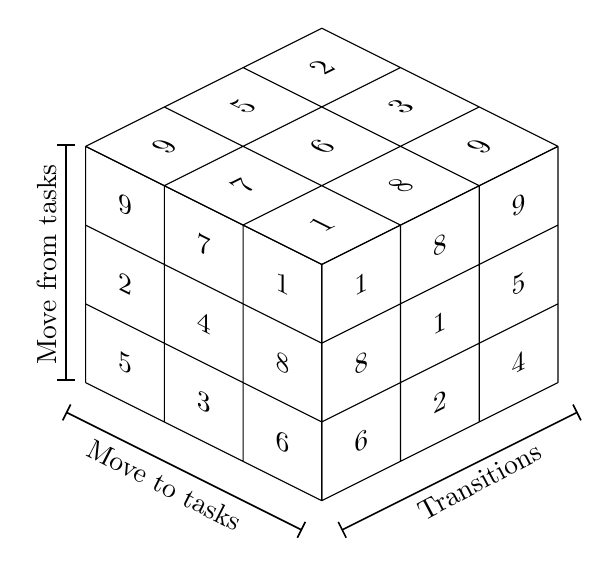
\begin{tikzpicture}
\begin{scope}[every node/.append style={yslant=-0.5},yslant=-0.5]
  \node at (0.5,2.5) {9};
  \node at (1.5,2.5) {7};
  \node at (2.5,2.5) {1};
  \node at (0.5,1.5) {2};
  \node at (1.5,1.5) {4};
  \node at (2.5,1.5) {8};
  \node at (0.5,0.5) {5};
  \node at (1.5,0.5) {3};
  \node at (2.5,0.5) {6};
  \draw (0,0) grid (3,3);
\end{scope}
\begin{scope}[every node/.append style={yslant=0.5},yslant=0.5]
  \node at (3.5,-0.5) {1};
  \node at (4.5,-0.5) {8};
  \node at (5.5,-0.5) {9};
  \node at (3.5,-1.5) {8};
  \node at (4.5,-1.5) {1};
  \node at (5.5,-1.5) {5};
  \node at (3.5,-2.5) {6};
  \node at (4.5,-2.5) {2};
  \node at (5.5,-2.5) {4};
  \draw (3,-3) grid (6,0);
\end{scope}
\begin{scope}[every node/.append style={
    yslant=0.5,xslant=-1},yslant=0.5,xslant=-1
  ]
  \node at (3.5,2.5) {9};
  \node at (3.5,1.5) {7};
  \node at (3.5,0.5) {1};
  \node at (4.5,2.5) {5};
  \node at (4.5,1.5) {6};
  \node at (4.5,0.5) {8};
  \node at (5.5,2.5) {2};
  \node at (5.5,1.5) {3};
  \node at (5.5,0.5) {9};
  \draw (3,0) grid (6,3);
\end{scope}

%x-axis
\draw[|-|,semithick,yslant=-0.5] (-0.25,-0.5) -- (2.75,-0.5);
\draw (1,-1.3) node[rotate= -27] {Move to tasks};

%y-axis
\draw[|-|,semithick,yslant=-0.5] (-0.25,-0.1) -- (-0.25,2.9);
\draw (-0.25,1.5) node[rotate=90, anchor= south] {Move from tasks};

%z-axis
\draw[|-|,semithick,yslant=-0.5] (3.25,-0.25) -- (6.25,2.75);
\draw (5,-1.25) node[rotate=28] {Transitions};
\end{tikzpicture}
\end{document} 

    	% or use \input{mytikz}
    	\caption{The timeMatrix3D}
    	\label{fig:3d_matrix}
   \end{figure}
 For the model to decide how long a move between two tasks should be and if there should be a change of tool in between, a matrix is used, $timeMatrix3D$, see figure \ref{fig:3d_matrix}. This is a 3-dimensional matrix and contains the times for moving between all the tasks depending on what tool change occurs. On its y-axis it has the tasks to move from, on the x-axis the tasks to move to, and on the z-axis the different transitions between tools that can occur.
 \begin{equation}\label{eq:timeMatrixDepth}
 timeMatrixDepth = \frac{n^2 - n + 2}{2}, \; n = nbrTools
 \end{equation}
  \begin{equation}
  \begin{aligned}\label{eq:44}
  timeMatrix3D(t(from),t(to),k) &\in \{0 , \ldots , 2^{32}-1\},\\
  t(from) &\in tasks \cup startTasks,  \\ 
  t(to) &\in tasks, \; k \in \{0 , \ldots , timeMatrixDepth\}
  \end{aligned}
  \end{equation}
 $timeMatrixDepth$ is the length of the z-axis, i.e. the depth of the matrix. It should be said that the reason for using the method described below is to reduce the size of the matrix and avoid too much redundancy.
 
 What we mean with ''different transitions'' is easiest to show through an example. Lets say we have $3$ tools available for each machine. We consider each tool state as a node in a graph, see figure \ref{fig:tools_trans_bef}, with the old tool state to the left and the new tool state to the right. Between them we can draw the different ways we can change state. The we start to consider which ones we actually need. We can change from tool $1$ to tool $1$, which is not changing tool at all. The same can be done for tool $2$, but not changing tool here costs just as much time as with tool $1$. So the change from tool $1$ to itself covers not changing tool for this tool, as well as for all the other tools, thereby we only need to keep track of one of these changes. We can also change from tool $1$ to tool $2$. And we can change back from $2$ to $1$, although here in the model we assume the change from one tool to another takes the same time the other way around as well. Therefore, we consider the change from tool $1$ to tool $2$ the same as from tool $2$ to tool $1$, and only keep track of one of them. If we keep consider the rest of the transitions this way, we will end up with a reduced number of transitions, in our case $4$, see figure \ref{fig:tools_trans_aft}
 
 It has been observed that using the reasoning above, $timeMatrixDepth$ follows the function \ref{eq:timeMatrixDepth}.
 
 \begin{figure}
 	\centering
 	\documentclass{standalone}
\usepackage{tikz}
\usetikzlibrary{calc, shapes, backgrounds}
\usepackage{standalone}
\usepackage{amsmath, amssymb}
\pagecolor{olive!50!yellow!50!white}
\begin{document}
\tikzset{
  leaf/.style = {draw=none,label = center:\textsf{$\vdots$}},
  labels/.style={midway, sloped, above, yshift=-10pt}
}
\begin{tikzpicture}
[
    scale = 0.75, transform shape, thick,
    every node/.style = {draw, circle, minimum size = 5mm, line width = 1pt, align=center},
    grow = down,  % alignment of characters
    level 1/.style = {sibling distance=6cm},
    level 2/.style = {sibling distance=2cm}, 
    level 3/.style = {sibling distance=1cm}, 
    level distance = 3 cm
  ]
  
  \tikzset{VertexStyle/.style = {shape          = circle,
                                   text           = black,
                                   inner sep      = 2pt,
                                   outer sep      = 5pt,
                                   minimum size   = 20pt}}
  \begin{scope}[node distance=20mm and 10mm]
  \node[VertexStyle](11){1};
  \node[VertexStyle, below of= 11](12){2};
  \node[VertexStyle, below of= 12](13){3};

  \node[VertexStyle, right= 2cm of 11](21){1};
  \node[VertexStyle, below of= 21](22){2};
  \node[VertexStyle, below of= 22](23){3};
  \end{scope}
  
  \draw(11) to (21);
  \draw(11) to (22);
  \draw(11) to (23);
  \draw(12) to (21);
  \draw(12) to (22);
  \draw(12) to (23);
  \draw(13) to (21);
  \draw(13) to (22);
  \draw(13) to (23);

\end{tikzpicture}
\end{document} 

 	% or use \input{mytikz}
 	\caption{All the transitions between the tool states}
 	\label{fig:tools_trans_bef}
 \end{figure}
 
 \begin{figure}
 	\centering
  	\documentclass{standalone}
\usepackage{tikz}
\usetikzlibrary{calc, shapes, backgrounds}
\usepackage{standalone}
\usepackage{amsmath, amssymb}
\pagecolor{olive!50!yellow!50!white}
\begin{document}
\tikzset{
  leaf/.style = {draw=none,label = center:\textsf{$\vdots$}},
  labels/.style={midway, sloped, above, yshift=-10pt}
}
\begin{tikzpicture}
[
    scale = 0.75, transform shape, thick,
    every node/.style = {draw, circle, minimum size = 5mm, line width = 1pt, align=center},
    grow = down,  % alignment of characters
    level 1/.style = {sibling distance=6cm},
    level 2/.style = {sibling distance=2cm}, 
    level 3/.style = {sibling distance=1cm}, 
    level distance = 3 cm
  ]
  
  \tikzset{VertexStyle/.style = {shape          = circle,
                                   text           = black,
                                   inner sep      = 2pt,
                                   outer sep      = 5pt,
                                   minimum size   = 20pt}}
  \begin{scope}[node distance=20mm and 10mm]
  \node[VertexStyle](11){1};
  \node[VertexStyle, below of= 11](12){2};
  \node[VertexStyle, below of= 12](13){3};

  \node[VertexStyle, right= 2cm of 11](21){1};
  \node[VertexStyle, below of= 21](22){2};
  \node[VertexStyle, below of= 22](23){3};
  \end{scope}
  
  \draw(11) to (21);
  \draw(11) to (22);
  \draw(11) to (23);
  \draw(12) to (23);

% \node (Start){}
%   child {   node [] (A) {}
%     child { node [] (D) {}
%       child { node [leaf] (M) {}}
%       child { node [leaf] (N) {}}
%     }
%     child { node [] (E) {}
%       child { node [leaf] (O) {}}
%       child { node [leaf] (P) {}}
%     }
%     child { node [] (F) {}
%       child { node [leaf] (Q) {}}
%       child { node [leaf] (R) {}}
%     }
%   }
%   child {   node [] (B) {}
%     child { node [] (G) {}
%       child { node [leaf] (S) {}}
%       child { node [leaf] (T) {}}
%     }
%     child { node [] (H) {}
%       child { node [leaf] (U) {}}
%       child { node [leaf] (V) {}}
%     }
%     child { node [] (I) {}
%       child { node [leaf] (X) {}}
%       child { node [leaf] (Y) {}}
%     }
%   }
%   child{ node(C){}
%     child { node [] (J) {}
%       child { node [leaf] (Z) {}}
%       child { node [leaf] (A1) {}}
%     }
%     child { node [] (K) {}
%       child { node [leaf] (B1) {}}
%       child { node [leaf] (C1) {}}
%     }
%     child { node [] (L) {}
%       child { node [leaf] (D1) {}}
%       child { node [leaf] (E1) {}}
%     }
%   };
\end{tikzpicture}
\end{document} 

  	% or use \input{mytikz}
  	\caption{The reduced number of transitions between the tool states}
  	\label{fig:tools_trans_aft}
 \end{figure}
 
 \begin{equation}\label{eq:56}
 taskOutOfRange(m) \subset tasks, \; m \in machines
 \end{equation}
Depending on the physical layout of the assembly, sometimes not all tasks can be done with all machines. It could be that the machines would collide or simply that the spatial location is out of reach for the machine. In those cases we can specify tasks are out of hand for a specific machine. This is the only time when we distinguish between the two machines and connect the machine in the model model with the machine in the real world. In all other aspects other than this the machines in the model are identical and has the potential perform the same work.
 
 
 \subsection{Decision variables}
 Decision variables are variables that can take on many values. It is these values that the solver set out to determine in order to solve the problem.
 
 \begin{equation}\label{eq:40}
 usingMachine(t) \in machines, \; t \in tasks
 \end{equation}
 The model has to decide which task uses which machine.
 
 \begin{equation}\label{eq:41}
 pred(t) \in allTasks, \; t \in allTasks
 \end{equation}
Each task has a predecessor that tells the model what other task comes right before the task in question on the same machine.
 
 \begin{equation}
 \begin{aligned}\label{eq:maxE}
 maxE = &(max(\{duration(t) : t \in tasks\}) \; +  \\ 
 &\begin{aligned}
 max(\{&timeMatrix3D(t_1,t_2,k) : \\
 &\forall t_1 \in tasks \cup startTasks,  \\ 
 &\forall t_2 \in tasks,\\
 &\forall k \in \{0 , \ldots , timeMatrixDepth\}\}) \times nbrTasks
  \end{aligned}
 \end{aligned}
 \end{equation}
 In order to create an upper limit for variables dealing with time, we create a rough upper limit of the complete assembly. It simply takes the longest duration for a task and the longest duration for a move between tasks and assert it for all the tasks.
 
 \begin{equation}\label{eq:46}
 start(t) \in \{0 , \ldots , maxE\}, \; t \in allTasks
 \end{equation} 
 \begin{equation}\label{eq:47}
 end(t) = start(t) + duration(t), \; t \in allTasks
 \end{equation}
Each task has to start have a start time. We set it to be anywhere between time $0$ and the maximum possible end calculated before.

To simplify notation we also introduce one more variable called $end(t)$. It is the time when task $t$ ends and is simply the sum of the start and the duration of the task.

 \begin{equation}\label{eq:49}
 moveDuration(t) \in \{0 , \ldots , maxE\}, \; t \in allTasks
 \end{equation}
 \begin{equation}\label{eq:50}
 moveStart(t) \in \{0 , \ldots , maxE\}, \; t \in allTasks
 \end{equation}
 \begin{equation}\label{eq:51}
 moveEnd(t) = moveStart(t) + moveDuration(t), \; t \in allTasks
 \end{equation}
As mentioned before, each task has a move time connected to it since it takes a certain amount of time to move from one task to another. Since this time depends on both what task comes before it and what tools is needed for both of the tasks, the duration for the move is a decision variable as opposed to the duration for the task itself.
 
 \begin{equation}\label{eq:48}
 makespan \in \{0 , \ldots , maxE\}
 \end{equation}
Since the goal of the assembly is to complete the assembly in as little time as possible, we set up a variable for it, $makespan$. It is this variable the solver will try to minimize.
 
 \begin{equation}\label{eq:52}
 toolUsed(t) \in tools, \; t \in allTasks
 \end{equation}
The last variable is for determine what tool should be used for a task. With $toolNeeded$ we specify what tool is needed for the specific task. But we do not need to specify a tool if the task does not need any specific tool. That is why we need to determine what tool should be used for those tasks. Leaving the option open by not specifying any particular tool opens up for optimisations since it could mean we can avoid costly tool changes.
  
 
 \section{Constraints}\label{seq:constraints}
 In this section some of the most important constraints for the model will be described. For a full list of used constraints see \emph{Appendix A}, for the MiniZink code see \emph{Appendix B}.
 
 \begin{equation}\label{eq:92}
 (\forall t \in tasks) \; end(t) \le makespan
 \end{equation}
$makespan$ should represent the total time of the whole assembly, since it is that which we want to minimize. That means it should be equal to the largest end time amongst all the tasks. We can enforce that by limiting the end time for each task to be less or equal to the $makespan$.
 
 \begin{equation}\label{eq:93}
 (\forall t \in startTasks \cup goalTasks) \; start(t) = 0
 \end{equation}
 \begin{equation}
 \begin{aligned}\label{eq:94}
 &(\forall m \in machines) \\
 &\begin{aligned}
 usingMachine(nbrTasks + m) &= m \; \land\\
 usingMachine(nbrTasks + nbrMachines + m) &= m
 \end{aligned}
 \end{aligned}
 \end{equation}
 Start and goal tasks are special tasks since they act as source and sink nodes. This means they never get scheduled in time as ordinary tasks, we set them to all start at time $0$ and they do not have a duration variable, since the do not take up any time. We also assign them to machines so each start and goal task pair have their own machine from the start.
 
 \begin{equation}\label{eq:95}
 \begin{aligned}
 (\forall m &\in machines) \\
 (\forall t &\in tasksOutOfRange(m)) \\
 usingMachine(t) &\neq m
 \end{aligned}
 \end{equation}
We enforce the $tasksOutOfRange(m)$ variables by simply saying that the tasks in the variable can not be assigned the machine $m$.

 \begin{equation}\label{eq:117}
 (\forall t \in tasks, \; toolNeeded(t) \neq 0) \; toolUsed(t) = toolNeeded(t)
 \end{equation}
 As said before, the $toolNeeded$ contains what tool is needed for a task. We need to translate it into what tool is used. It is done by simply taking the value from $toolNeeded$ and assign it to $toolUsed$ for the tasks where a tool is specified, i.e. $toolNeeded$ is not $0$.
 
 \subsection{Precedences}
 These constraints deals with the order in time in which the tasks as to come.
 
  \begin{equation}\label{eq:107}
  (\forall t \in tasks) \; Start(t) \geq moveEnd(t)
  \end{equation}
A very fundamental part of the relation between a task and the move to it is that we cannot start a task before we have moved to it.
 
 \begin{equation}
 \begin{aligned}\label{eq:96}
 (\forall comp &\in components) \\
 (\forall mountTask &\in mounting(comp)) \\
 (\forall putTask &\in putting(comp)) \\
 end(putTask) &\le moveStart(mountTask)
 \end{aligned}
 \end{equation}
 If we want to mount two components together, we first have to put the first component in a fixture before we can mount the other component on it. Hence, the put task has to end before we can start with the mount task. 
 
 \begin{equation}
 \begin{aligned}\label{eq:97}
 \forall comp &\in components \\
 \forall mountTask &\in mounting(comp), \\
 \forall takeTask &\in taking(comp), \\
 end(takeTask) &\le moveStart(mountTask)
 \end{aligned}
 \end{equation}
 In the case mentioned above we also have take tasks for both components and they must both be performed before we can start mounting anything. 
 
 \begin{equation}
 \begin{aligned}\label{eq:98}
 \forall comp &\in components \\
 (\forall putTask &\in putting(comp), \; tray(putTask) > 0)\\
 (\forall takeTask &\in taking(comp), \; tray(putTask) = tray(takeTask))\\
 end(putTask) &\le moveStart(takeTask)
 \end{aligned}
 \end{equation}
 Say we want to put a component away for a while and pick it up again later. Then we need to do that in a tray. This is the only time we put anything in a tray, usually we just take components from them. So we can apply the \ref{eq:98} constraint which says that if there is a take and a put on the same tray, then the take has to happen after the put. 
 
 \begin{equation}
 \begin{aligned}\label{eq:99}
 (\forall f &\in fixtures) \\
 (\forall putTask &\in putting, \; fixture(putTask) = f)\\
 (\forall takeTask &\in taking, \; fixture(takeTask) = f \; \land \\
 &componentsUsed(putTask) \subset taskSubComponents(takeTask)) \\
 end(putTask) &\le moveStart(takeTask), \\
 \end{aligned}
 \end{equation}
 When there is a put task and a take task on a fixture where a sub-component of the component being taken is the component being put, the put task has to happen before the take task.
 
 \begin{equation}
 \begin{aligned}\label{eq:100}
 &(\forall f \in fixtures) \\
 &puts = [put : \forall put \in putting, \; fixture(put) = f], \\
 &\begin{aligned}
 takes = [min(\{&take : \forall take \in taking, \; fixture(take) = f,\\ &componentsUsed(put) \subset taskCompleteSubComponent(take)\}) : \\
 &\forall put \in puts], 
 \end{aligned}\\
 &\begin{aligned}
 cumulative(&[moveStart(task) : \forall task \in puts], \\ &[abs(end(takes(i))-moveStart(puts(i))) : \forall i \in \{1 , \ldots , |puts|\}], \\
 &[1 : \forall i \in \{1 , \ldots , |puts|\}],\\
 &1)
 \end{aligned}\\
 \end{aligned}
 \end{equation}
 Since we can do many sub-assemblies on the same fixture, we need to ensure that if a component is put in the fixture, there cannot be a component from another sub-assembly put or mounted there before the sub-assembly is done.
 
 We can observe that the task of doing a sub-assembly begins with a put of a component in a fixture and a take of a component from the same fixture. The taken component will have the put component as a sub-component. With this knowledge we start by extracting all put tasks for a fixture. Then we extract all the corresponding take tasks, i.e. the take tasks for that fixture where the component used in the put task is among the sub-components for the component in the take task. Although, there is the case where we construct a component by first doing some mounting, then we take it up to maybe turn it or fixate it, and then put it back in the fixture for further mounting. In this case we will get two takes matching with the first put. So we need to identify which take task is the first one. We do this by choosing the take task with the least amount of subcomponents.
 
 Now we have a 1:1 matching of take tasks and put tasks. To ensure the time between when a put task occurs and when the take task occurs, we apply a \emph{cumulative} constraint over that time and the limit of the fixture is always $1$.
 
 \begin{equation}
 \begin{aligned}\label{eq:101}
 (\forall group &\in \{1 , \ldots , nbrConcurrentGroups\}) \\
 (\forall t_1 &\in concurrentTasks(group)) \\
 (\forall t_2 &\in concurrentTasks(group) / \{t_1\}) \\
 start(t_1) &= start(t_2) \; \land \\
 usingMahine(t_1) &\neq usingMachine(t_2), \\
 \end{aligned}
 \end{equation}
 The fundamental property of the tasks in a concurrent group is that they need to execute at the same time on different machines. We ensure this with \ref{eq:101}.
 
 \begin{equation}
 \begin{aligned}\label{eq:102}
 (\forall t_1 &\in tasks, \; componentCreated(t1) > 0) \\
 (\forall t_2 &\in tasks, \; componentCreated(t_1) \in compinentUsed(t_2)) \\
 moveStart(t_2) &\geq end(t_1) \\
 \end{aligned}
 \end{equation}
 A very logical observation we can do is that components cannot be used before they are created. This is enforced in \ref{eq:102}.
 
 \begin{equation}
 \begin{aligned}\label{eq:103}
 (\forall precTask &\in tasks) \\
 (\forall t &\in tasks, \; precTask \neq t,\\
 &componentUsed(precTask) \cup taskCompleteSubComponent(t) \subset\\
 &taskCompleteSubComponents(t),\\
 &componentsUsed(precTask) \cup taskCompleteSubComponents(t) \neq \emptyset)\\
 end(precTask) &\leq moveStart(t), \\
 \end{aligned}
 \end{equation}
 A similar observation as for \ref{eq:102} is that we have to perform all tasks with a component before it is part of a sub-assembly. Therefore we can say that all tasks needs to have an end time smaller than the start time of the tasks having the tasks component as sub-component.
 
 \begin{equation}
 \begin{aligned}\label{eq:104}
 &\begin{aligned}
 (\forall f &\in fixtures) \\
 fixtureTasks &= [t : \forall t \in tasks, \; fixture(t) = f], 
 \end{aligned}\\
 &\begin{aligned}
 cumulative(&[start(t) : \forall t \in fixtureTasks],\\
 &[duration(t) : \forall t \in fixtureTasks],\\
 &[1 : t \in fixtureTasks],\\
 &1)
 \end{aligned}\\
 \end{aligned}
 \end{equation}
 \begin{equation}
 \begin{aligned}\label{eq:105}
 &\begin{aligned}
 (\forall tr &\in trays) \\
 trayTasks &= [t : \forall t \in tasks, \; tray(t) = tr], 
 \end{aligned}\\
 &\begin{aligned}
 cumulative(&[start(t) : \forall t \in trayTasks],\\
 &[duration(t) : \forall t \in trayTasks],\\
 &[1 : t \in trayTasks],\\
 &1)
 \end{aligned}\\
 \end{aligned}
 \end{equation}
 \begin{equation}
 \begin{aligned}\label{eq:106}
 &\begin{aligned}
 (\forall o &\in outputs) \\
 outputTasks &= [t : \forall t \in tasks, \; output(t) = o], \\
 \end{aligned}\\
 &\begin{aligned}
 cumulative(&[start(t) : \forall t \in outputTasks], \\
 &[duration(t) : \forall t \in outputTasks], \\
 &[1 : t \in outputTasks], \\
 &1)
 \end{aligned}\\
 \end{aligned}
 \end{equation}
Trays, fixtures and outputs can only be used one at a time. We can rephrase this into saying that tasks using trays cannot overlap, tasks using fixtures cannot overlap, etc. We ensure this by applying the \emph{cumulative} constraint through \ref{eq:104}, \ref{eq:105} and \ref{eq:106}.
 
 \newpage
 \subsection{Predecessors}
 \begin{equation}\label{eq:109}
 \begin{aligned}
 (\forall startTask &\in startTasks / \{nbrTasks + 1\}) \\
 pred(startTask) &= startTask + nbrMachines - 1
 \end{aligned}
 \end{equation}
 \begin{equation}\label{eq:110}
 pred(nbrTasks + 1) = nbrTasks + nbrMachines \times 2
 \end{equation}
 \begin{equation}\label{eq:111}
 circuit(\{pred(t) : \forall t \in tasks\})
 \end{equation}
 All tasks has to have a predecessor that tells the model what task comes directly before said task on the same machine. This means that a task can only have one predecessor. It can be seen as the way a machine needs to travel through its tasks in order to complete the assembly, where we have a start task at the start and a goal task at the end. If we were to connect the start and the goal task we wold have a circuit, hence we could view each machine as a circuit. And we could model each machine as a circuit, but then we would need to synchronise all the sub-circuits and ensure that tasks only appeared in one sub-circuit. This would make for quite a few constraints and would make the model more complex. Instead we model all the machines as one circuit and we tie together the goal task of one sub-circuit with the start task of the next for each sub-circuit, to form a large circuit. Then we tie together the goal task of the last sub-circuit with the start task of the first, see \ref{eq:110}. Lastly we can apply the \texttt{circuit} constraint over all $pred$ variables.
 
The attentive reader might have observed that the nodes in the \texttt{circuit} constraint have successors and not predecessors. Even if it is the wrong way around, it does not matter if the constraint sees the predecessor variable as a successor or a predecessor, it will form a circuit anyway.
 
 \begin{equation}\label{eq:108}
 (\forall t \in tasks) \; moveStart(t) \geq end(pred(t))
 \end{equation}
A fundamental part of a predecessor is that it is the task directly before the task in question, therefore the predecessor has to end before the task starts, or more specific, even before the move to the task.
 
 \begin{equation}\label{eq:115}
 \begin{aligned}
 (\forall t &\in tasks \cup goalTasks) \\
 usingMachine(t) &= usingMachine(pred(t)) 
 \end{aligned}
 \end{equation}
Another fundamental part is that a predecessor is a task performed on the same machine as the task in question. This is enforced by \ref{eq:115}.

 \begin{equation}
 \begin{aligned}\label{eq:114}
 &\begin{aligned}
 (\forall k &\in orderedGroups) \\
 (\forall i &\in \{1 , \ldots , |orderedGroup(k)|-1\}) 
 \end{aligned}\\
 &pred(ordered(k, i + 1)) = ordered(k, i) \\
 \end{aligned}
 \end{equation}
In a sense, the ordered groups are forced predecessors and hence we enforce that by simply by making a task predecessor to the next task in the array.
\\\\
The following two constraints can seem very specific, but are essential to the scheduling in our model.
 \begin{equation}
 \begin{aligned}\label{eq:112}
 (\forall c &\in components) \\
 (\forall mountTask &\in mounting(c)) \\
 puts &= \{p : \forall p \in putting(c),\\
 &(fixture(p) > 0 \land fixture(p) = fixture(mountTask)) \; \lor  \\
 &(output(p) > 0 \land output(p) = output(mountTask)), \\
 (\forall takeTask &\in taking(c), \; takeTask \notin orderedSet, \; puts = \emptyset) \\
 pred(mountTask) &= takeTask \\
 \end{aligned}
 \end{equation}
 In order to properly connect the taking of a component and the mounting of one, we need to ensure that if there is no put task, the take task has to be the predecessor of the mount task. 
 
 But we must also ensure the following: The put cannot be on the same fixture or output as the mount. This is because a component that will be mounted in a fixture or output will always first be picked up, then put in either a fixture or output, then mounted with with another component. The component mounted on will also be part of the mounting task. Therefore, if the component is the one being mounted, there will be two tasks; one where the component is taken, and one where the component is mounted. And that is no problem, the constraint applies. But if the component is the one being mounted on, there will be three tasks; one where the component is taken, one where the component is put in a fixture or output, and one where it is mounted on. In this case the take task cannot be the predecessor of the mount task, since the component first must be put in the fixture or output, and then the other take task,  where the component being mounted on this component is taken, should be the predecessor of the mount task. Hence we ensure there are no put tasks working on the same fixture or output as the mount task.
 
 The final case we must consider is when there are move tasks involved. There can be a case of a take task of a component, then a couple of move tasks, and lastly a mount task. In this case, the take task cannot be the predecessor of the mount task, and this constraint does not apply. If we applied it, it would contradict the \ref{eq:114} constraint. So we need to ensure the take task is not in an ordered group either.
 
 \begin{equation}
 \begin{aligned}\label{eq:113}
 (\forall c &\in components, \; moving(c) = \emptyset)\\
 (\forall putTask &\in putting(c), \; tray(putTask) = 0)\\
 (\forall takeTask &\in taking(c))\\
 pred(putTask) &= takeTask
 \end{aligned}
 \end{equation}
 As with \ref{eq:112}, in order to ensure the relation between when a component is picked up and when it is put that the take task is the predecessor of the put task, i.e. we must first pick up the components before we put it down, and there cannot be anyu other task in between.
 
 Also as with \ref{eq:112}, there are a few cases to consider. If we want to put a component away for a while in order to pick it up later, there will be a put task and a take task on that component. But in this case the take task cannot come before the put task, since we need to put it down before we can pick it up. So we put in the clause that this constraint does not apply if the put task is on a tray.
 
 We also need to consider the occurrence of move tasks. If there is a move task involved between the take and put, the take task cannot be the predecessor of the put task.
 
 \begin{equation}\label{eq:116}
 \begin{aligned}
 (\forall t &\in tasks) \\
 k &= abs(toolUsed(t) - toolUsed(pred(t))) + 1, \\
 moveDuration(t) &= timeMatrix3D(pred(t), \; t, \; k)
 \end{aligned}
 \end{equation}
\ref{eq:116} is the constraint that decides if there should be a tool change or not between two tasks. It first calculates what tool state transition will occur between the two tasks, $k$, by taking the difference between what tool is used in the task and its predecessor. If they use the same tool, no transition needs to occur, i.e. no tool change needed and the difference would be $0$. We add $1$ to $k$ since the indexes start at $1$ in \emph{MiniZinc} and a result of $0$ should take constraint to the first index dept-wise in the $timeMatrix3D$.
 

 
 
 \section{Filter}
  In \cite{VilimBartak2002Batch} \cite{Vilim2002Precedence} \cite{VilimBartak2002Sequence} Vilím shows that filtering the domains of variables when, as in our case, using sequence dependent setup times can have a great effect on the runtime. Here we present a set of filters in order to minimize the domains of the variables.
  
\subsection{Temporal filter}
  The largest domains in the model are the domains for the variables dealing with time, i.e. the temporal variables. Reducing those has the potential to cut much of the processing time.
  
  \begin{equation}
  \begin{aligned}\label{eq:57}
  &( \forall t \in tasks)\\
  &\begin{aligned}
  maxMoveDurs(t) = max(\{&timeMatrix3D(t,j,k) :\\
  &\forall j \in tasks, \\
  &\forall k \in \{1 , \ldots , timeMatrixDepth\},\\
  &j \neq t\})
  \end{aligned}
  \end{aligned}
  \end{equation}
   \begin{equation}
   \begin{aligned}\label{eq:58}
   &(\forall t \in tasks)\\
   &\begin{aligned}
   minMoveDurs(t) = min(\{&timeMatrix3D(t,j,k) :\\
   &\forall j \in tasks, \\
   &\forall k \in \{1 , \ldots , timeMatrixDepth\},\\
   &j \neq t\})
   \end{aligned}
   \end{aligned}
   \end{equation}
 We start with defining two variables, $maxMoveDurs(t)$ and $minMoveDurs(t)$. These contain the maximum duration and the minimum duration respectively for each task taken from the time matrix.
  
  \begin{equation}\label{eq:59}
 	maxEnd = \sum_{\forall t \in tasks} duration(t) + maxMoveDurs(t)
  \end{equation}
  \begin{equation}\label{eq:minEnd}
  	minEnd = \frac{\sum_{\forall t \in tasks} duration(t) + minMoveDurs(t)}{nbrMachines}
  \end{equation}
 By using the newly created variables we candefine yet another two. These define a new maximum for the total time of the assembly, $maxEnd$. It is similar to $maxE$ in equation \ref{eq:maxE}, although much more thorough in the filtering. These variables also define a new minimum for the total time of the assembly, it was earlier ju set to 0.
 
 To calculate the maximum end we look at the worst case scenario for the assembly. The worst case would be if all the tasks had to be done one after the other, one at a time, on the same machine and they would take the longest time, according to the time matrix, to move between them. See figure \ref{fig:worst_case}. This can simply be defined by summing the durations and maximum move durations for all the tasks.
 
 To calculate the minimum end we look at the best case scenario. The best case scenario is if all the tasks can be evenly scheduled over all machines, taking the shortest, according to the time matrix, time to move between them. See figure \ref{fig:best_case}. We can define this by summing up the durations and minimum move durations for all the task end divide the sum with the number of machines available. If the tasks can be perfectly evenly scheduled across all the machines, the total assembly time will be equal to $minEnd$, if they cannot $minEnd$ will always be smaller than the total assembly time.
 
  \begin{figure}
  	\centering
  	\documentclass{standalone}
\begin{document}

\sffamily
\begin{tikzpicture}[
  thick,
  myrect/.style={
    draw,
    rectangle split,
    rectangle split horizontal,
    rectangle split parts=#1,
    rectangle split part align=center
    } 
]

\node[myrect=6, anchor=west](assembly)
  {
  \nodepart[text width= 17mm]{one}$m_1$
  \nodepart[text width= 15mm]{two}$t_1$
  \nodepart[text width= 12mm]{three}$m_2$
  \nodepart[text width= 11mm]{four}$t_2$
  \nodepart[text width= 18mm]{five}$m_3$
  \nodepart[text width= 20mm]{six}$t_3$
  };
  
      % Draw axes
      \draw[thick,->] (0,-1) -- (0,1);
      \draw[thick,->] (0,-1) -- (12,-1);

\end{tikzpicture}

\end{document} 

  	% or use \input{mytikz}
  	\caption{The worst case assembly}
  	\label{fig:worst_case}
  \end{figure}
   \begin{figure}
   	\centering
   	\documentclass{standalone}
\begin{document}

\sffamily
\begin{tikzpicture}[
  thick,
  myrect/.style={
    draw,
    rectangle split,
    rectangle split horizontal,
    rectangle split parts=#1,
    rectangle split part align=left
    } 
]

\node[myrect=2,anchor=west](assembly)
  {
  \nodepart[text width= 17mm]{one}$m_1$
  \nodepart[text width= 15mm]{two}$t_1$
  };
  
\node[myrect=2, below =of assembly.west,anchor=west](assembly2)
  {
  \nodepart[text width= 12mm]{one}$m_2$
  \nodepart[text width= 11mm]{two}$t_2$
  };
  
\node[myrect=2, below=of assembly2.west,anchor=west](assembly3)
  {
  \nodepart[text width= 18mm]{one}$m_3$
  \nodepart[text width= 20mm]{two}$t_3$
  };
  
      % Draw axes
      \draw[thick,->] (0,-3) -- (0,1);
      \draw[thick,->] (0,-3) -- (5,-3);

\end{tikzpicture}

%\begin{tikzpicture}
%\tikzset{VertexStyle/.style = {anchor= west, draw, align= center, text height= 2.5mm}
%}
%
%    % Draw axes
%    \draw [<->,thick] (0,4) node (yaxis) [above] {}
%        |- (45mm,0) node (xaxis) [right] {};
%
%   \node[VertexStyle, text width= 15mm] (rect1) at (0mm,3)  {$m_1$};
%   \node[VertexStyle, text width= 15mm] (rect2) at (18mm,3) {$t_1$};
%   
%   \node[VertexStyle, text width= 10mm] (rect1) at (0mm,2)  {$m_2$};
%   \node[VertexStyle, text width= 11mm] (rect2) at (13mm,2) {$t_2$};
%      
%   \node[VertexStyle, text width= 11mm] (rect1) at (0mm,1)  {$m_3$};
%   \node[VertexStyle, text width= 20mm] (rect2) at (14mm,1) {$t_3$};
%\end{tikzpicture}
\end{document} 

   	% or use \input{mytikz}
   	\caption{The best case assembly}
   	\label{fig:best_case}
   \end{figure}
 \newpage
 We can now start using $maxEnd$ and $minEnd$ to filter variables
  \begin{equation}\label{eq:lim_start_over}
  \begin{aligned}
 &(\forall t \in allTasks)\\
 &start(t) \le maxEnd-duration(t)
  \end{aligned}
  \end{equation}
   \begin{equation}\label{eq:lim_start_under}
  \begin{aligned}
 &(\forall t \in Tasks)\\
 &start(t) \ge minMoveDurs(t)
  \end{aligned}
  \end{equation}
 We set and upper bound for the start of a task by setting it to happen at latest the duration of the task time units before the $maxEnd$, since the task has to have time to execute before the end.
 
 To set a lower bound for the start of a task, we simply reason that the move to the task can start at its earliest at time 0. Therefore, we limit the task to start earliest direct after the minimum move duration to it.
 
 The difference between \ref{eq:lim_start_over} and \ref{eq:lim_start_under} is that the upper limit can be set for all sorts of tasks, even the start and goal tasks, but the lower limit cannot be set for start and goal tasks. This is simply because the start and goal tasks do not have any move times to them since they are source and sink nodes.
 
  \begin{equation}\label{eq:63}
  (\forall t \in tasks) \; moveStart(t) \le maxEnd-(duration(t)+minMoveDurs(t))
  \end{equation}
  In order to limit the move start to a task we use the same reasoning as with start. But now we have to account for that there comes a task after the move and a duration of the move itself. So we have to subtract the duration of the task and the duration of the move. Since we do not know the exact length of the move, we have to use the value we know the duration can not be lower than, which is $minMoveDuration$.
  
  \begin{equation}\label{eq:66}
  \begin{aligned}
  makeSpan &\le maxEnd \land\\
  makespan &\ge minEnd
  \end{aligned}
  \end{equation}
  We have already calculated the limits for the whole assembly, $maxEnd$ and $minEnd$. Now we just enforce them on the makespan.
  
  \begin{equation}
  \begin{aligned}\label{eq:67}
  &(\forall t \in tasks)\\
  &\begin{aligned}
  (\forall i \in \{0 , \ldots , maxMoveDurs(t)\} / \{&timeMatrix3D(task,j,k) :\\
  &\forall j \in tasks,\\
  &\begin{aligned}
  &\forall k \in \{1 , \ldots , timeMatrixDepth\}\\
  &t \neq j\})
  \end{aligned}
  \end{aligned}\\
  &moveDuration(t) \neq i
  \end{aligned}
  \end{equation}
 We know that the value for move duration will be one of the values in the time matrix, hence we can restrict the duration to only those values. We do that by coming up with the values that the duration cannot assume, and limits the duration to not have those values in its domain.
  
  \begin{equation}
  \begin{aligned}\label{eq:69}
  &(\forall t \in tasks / taking) \\
  &moveStart(t) \ge min(\{duration(tt) + minMoveDurs(tt) : \forall tt \in taking\})
  \end{aligned}
  \end{equation}
  The first thing that has to happen to a component in the assembly is that is has to be picked up. So since the assembly starts out with empty machines the first thing that has to happen, with the exception of a tool change, is a take task. Therefore, we can limit that start of the tasks not being take tasks to happen at earliest after the task with the smallest sum of duration and minimum move duration.
  
  \begin{equation}
  \begin{aligned}\label{eq:70}
  &(\forall t \in tasks)\\
  &\begin{aligned}
  prevTasks = \{task : &\forall task \in tasks,\\
  &componentCreated(task) \in componentsUsed(t)\},
  \end{aligned}\\
  &\begin{aligned}
  nbrMachines &\ge |prevTasks|,\\
  0 &< |prevTasks|,
  \end{aligned}\\
  &start(t) \ge max(\{duration(pt) + minMoveDurs(pt) : \forall pt \in prevTasks\}) \\
  \end{aligned}
  \end{equation}
  The start of a task can be even further limited by analysing the components used by the task and how that relates to what components are created by other tasks.
  
  Lets take task $t$ as an example. We start by getting all tasks that creates the components that is used in task $t$, $prevTasks$. These tasks has to come before task $t$ since the component that they create cannot be used before they are created. If the number of machines are greater than or equal to the number of task preceding task t, then the best scheduling that can be done is to do all tasks in parallel. That means that task $t$ can start at earliest after the one of the proceeding tasks taking the longest to complete.
  
  \begin{equation}
  \begin{aligned}\label{eq:71}
  &(\forall t \in tasks) \\
  &\begin{aligned}
  prevTasks = \{task : &\forall task \in tasks,\\
  &componentCreated(task) \in componentsUsed(t)\},
  \end{aligned} \\
  &nbrMachines < |prevTasks|,  \\
  &start(t) \ge \frac{\left(\sum_{\forall pt \in prevTasks}duration(pt) + minMoveDurs(pt)\right)}{nbrMachines}
  \end{aligned}
  \end{equation}
  But if the number of machines is fewer than the number of preceding tasks, the best we can do is divide them as equally as possible over the machines. This is the same reasoning as when we calculated $minEnd$ in equation \ref{eq:minEnd}.
  
  \begin{equation}\label{eq:72}
  \begin{aligned}
  &(\forall t \in tasks) \\
  &succTasks = \{task : \forall task \in tasks,\\
  &componentsUsed(t) \subset taskCompleteSubComponent(task), \\
  &componentsUsed(t) \cup taskCompleteSubComponents(task) \neq \emptyset\}, \\
  &\begin{aligned}
  nbrMachines &\ge |succTasks|,\\
  0 &< |succTasks|,
  \end{aligned}\\
  &\begin{aligned}
  start(t) \le maxEnd - max(\{&duration(st) + minMoveDurs(st) :\\
  &\forall st \in succTasks\}) - duration(t)
  \end{aligned}\\
  \end{aligned}
  \end{equation}
  To set the upper limit for the start of tasks we use a little bit different strategy.
  
  We know that if a component $c$ has been mounted on another component, $c$ cannot be used again on its own. Therefore, a task that uses component $c$ has to come before the tasks that uses a component in which $c$ is a part of.
  
  We use the same strategy as in \ref{eq:70} and look at the best case scenario where the tasks are performed concurrently on all machines. The difference here from \ref{eq:70} is that here we have to look at the maximum end of the assembly and subtract the successor task which takes the longest to perform and the duration of the task in question.
  
  \begin{equation}\label{eq:73}
  \begin{aligned}
  &(\forall t \in tasks)\\
  &succTasks = \{task : \forall task \in tasks, \\
  &componentsUsed(t) \subset taskCompleteSubComponent(task), \\
  &componentsUsed(t) \cup taskCompleteSubComponents(task) \neq \emptyset\}, \\
  &nbrMachines \le |succTasks|, \\
  &\begin{aligned}
  start(t) \; \le \; &maxEnd - \frac{\left(\sum_{\forall st \in succTasks}duration(st) + minMoveDurs(st)\right)}{nbrMachines}\\
  &- duration(t)
  \end{aligned}
  \end{aligned}
  \end{equation}
  As with \ref{eq:71} we look at the worst case scenario.
  
  
  \subsection{Predecessor filter}
  Since the predecessors are searched by the solver before searching the start variables, reducing their domains has potential to help reduce the total runtime considerably.
 
  \begin{equation}\label{eq:75}
  (\forall t1, \forall t2 \in taking) \; pred(t1) \neq t2
  \end{equation}
  \begin{equation}\label{eq:76}
  (\forall t1, \forall t2 \in putting \cup mounting) \; pred(t1) \neq t2
  \end{equation}
 In our model the tools can only pick up one component at a time. This also means that if a task puts down a component or mounts one, there cannot be a mount or put task directly afterwards.
  
  \begin{equation}
  \begin{aligned}\label{eq:78}
  &(\forall t \in tasks)\\
  &nonPredecessors = \{t_2 : \forall t_2 \in tasks, \\
  &componentsUsed(t) \subset taskCompleteSubComponents(t_2) \; \lor \\
  &componentsUsed(t) \subset subComponents(componentCreated(t_2))\} \\
  &(\forall nonPred \in nonPredecessors) \\
  &pred(t) \neq nonPred, \\
  \end{aligned}
  \end{equation}
  Using a similar reasoning as in \ref{eq:72} and \ref{eq:73}, we can find the tasks that cannot be the predecessor of task $t$. We look at what tasks uses the components that has the components used in $t$ as sub-components. This means that those components cannot come before task $t$, and therefore cannot be predecessors of $t$.
  
  \begin{equation}\label{eq:79}
  \begin{aligned}
  &(\forall startTask \in startTasks)\\
  &(\forall putTask \in putting)\\
  &pred(putTask) \neq startTask
  \end{aligned}
  \end{equation}
  \begin{equation}\label{eq:80}
   \begin{aligned}
   &(\forall startTask \in startTasks)\\
   &(\forall mountTask \in mounting)\\
   &pred(mountTask) \neq startTask 
   \end{aligned}
  \end{equation}
  As mentioned before, a component has to be picked up first before it can be manipulate in any way and the assembly has to start with a take task. Therefore, we can say that an assembly cannot start with neither a put task nor a mount task.
  
  The same could be said for move tasks, but since they need to be in an ordered group, a constraint like these would no make any difference.
  
  \begin{equation}\label{eq:81}
  \begin{aligned}
  &(\forall goalTask \in goalTasks) \\
  &(\forall takeTask \in taking) \\
  &pred(goalTask) \neq takeTask
  \end{aligned}
  \end{equation}
  The same way we can observe that an assemble needs to start with a take task, we can observe that an assembly cannot end with a take task. There is no component in the assembly that does not end up in the finished assembly, therefore the assembly cannot end with a machine holding a component, since it needs to be on the output in some way. 
  
  \begin{equation}
  \begin{aligned}\label{eq:82}
  &\begin{aligned}
  counts &= \{i : \forall task \in outputTasks, \; i \in \{0 , \ldots , 1\}\}, \\
  outputTasks &= \{task : \forall task \in tasks, \; output(task) > 0\}, \\
  goalPreds &= \{pred(task) : \forall task \in goalTasks\},
  \end{aligned} \\
  &global\_cardinality(goalPreds, \; outputTasks, \; counts) \; \land\\
  &\sum counts > 0
  \end{aligned}
  \end{equation}
   \begin{equation}
   \begin{aligned}\label{eq:83}
   &\begin{aligned}
   counts &= \{i : \forall task \in startTasks, \; i \in \{0 , \ldots , 1\}\}, \\
   takePreds &= \{pred(task) : \forall task \in taking\}, 
   \end{aligned}\\
   &global\_cardinality(takePreds, \; startTasks, \; counts) \; \land\\
   &\sum counts > 0
   \end{aligned}
   \end{equation}
 Continuing the reasoning around what tasks can come first and not we can expand with which tasks has to come last. We cannot limit the last task on each arm to be on an output, because it does not necessarily need to be that. Although, among the last tasks in the assembly there needs to be a task on an output. We can easily check that by placing a constraint over the $pred$ variables for the goal tasks. This is what \ref{eq:82} says.
 
 We can do the same reasoning with what needs to come first in the assembly. As we stated before, a take task has to be the first task in the assembly. And as with the last tasks in the assembly, the first task of a machine does not have to be a take task, but there needs to be at least one take task among the first tasks. We ensure this in \ref{eq:83} by placing a constraint over the $pred$ variables for the take tasks.